\documentclass[12pt]{article}
    \usepackage[a4paper,margin=1in]{geometry}
    \usepackage{setspace}
    \usepackage{amsmath}
    \usepackage{amssymb}
    \usepackage{graphicx}
    \usepackage{booktabs}
    \usepackage{makecell}
    \usepackage{graphicx}
    \usepackage{tabularx}
    \usepackage{float}
    \usepackage{xurl}
    \usepackage[hidelinks]{hyperref}

    %TC:envir table 0 0
    %TC:envir figure 0 0
    %TC:envir tabularx 0 0
    
    \doublespacing
     
    \begin{document}
    
    %TC:ignore
    \begin{center}
    \textbf{Linear regression models to estimate NVIDIA's stock close price}
    \end{center}
    
    \vspace{1em}
    
    \begin{center}
    \textbf{To what extent can linear regression models reliably estimate NVIDIA's stock close price?}
    \end{center}
    
    \vspace{1em}
    
    \begin{center}
    \textbf{IB Subject: Economics SL}
    
    \vspace{1em}
    
    \textbf{Word count: 3996} \\
    \textbf{Candidate Code: MKT963} \\
    \textbf{Citation Style: APA 7th Edition } \\
    \textbf{Session: May 2026}
    \end{center}
    
    \vspace{2em}
    
    \newpage
    
        \renewcommand{\contentsname}{Table Of Contents}
        
        \tableofcontents
    
    %TC:endignore
    \newpage
    
    \section{Introduction:}
    
    While NVIDIA's extraordinary growth during the AI boom has captivated investors, accurately estimating the price of such volatile tech stocks remains one of the most challenging problems in financial economics. In economic terms, NVIDIA's stock price is determined by the interaction of supply and demand in equity markets, where price signals aggregate the expectations of millions of investors regarding future profitability. These expectations are shaped by a wide range of variables: the derived demand for GPUs driven by AI adoption, the cost of raw material inputs such as copper and rare earth metals, and broader macroeconomic conditions reflected in market indices. This investigation therefore asks: to what extent can linear regression models reliably estimate NVIDIA's stock close price?
    
    \vspace{1em}
    
    Although more advanced machine learning models, such as neural networks, can achieve high estimative accuracy, they require extensive computational resources and hyperparameter tuning that would shift the focus of this essay away from economic analysis. Linear regression models were therefore selected due to their interpretability, methodological transparency, and suitability for evaluating the relative economic significance of estimator variables within the scope of this Extended Essay.
    
    \vspace{1em}
    
    To address the question, seven linear regression models are constructed. These models are grouped into three categories: sector-linked variables, commodity-linked variables, and broader market indicators. Sector-linked variables include major semiconductor firms and emerging small modular reactor companies. Commodity-linked variables include yearly metal production, metal futures prices, and metal exchange-traded funds. Broader market indicators include the Nasdaq 100 and the S\&P 500. Each model uses lagged estimator variables to estimate NVIDIA's stock close price the following day. The resolution of metal production is yearly due to limitations in data availability.
    
    \vspace{1em}
    
    Each model is evaluated using diagnostic and performance tests. The Breusch--Pagan and White tests are applied to detect heteroskedasticity, the Variance Inflation Factor (VIF) for multicollinearity, and the Durbin-Watson test for autocorrelation. Model performance is primarily compared using the adjusted $R^2$ to measure explanatory power.
    
    \section{Methodology:}

    \subsection{Linear Regression Models:}
    
    To estimate the stock price, Linear Regression Models (LRMs) are used. As Gujarati (2011) explains, LRMs are statistical tools used to model the relationship between data points, for example, the relationship between the price of a good and the cost of its raw material inputs. In this investigation, LRMs model the relationship between NVIDIA's stock closing price and the variables that theoretically drive it through economic mechanisms such as input cost transmission, sector interdependence, and market sentiment. They work as follows:
    
    $
    Y_i = \beta_1 X_1 + \beta_2 X_2 + \beta_3 X_3 + \beta_4 X_4 + \cdots + \beta_{ki} X_{ki} + u_i
    $
    
    Where $Y$ is the regressand (NVIDIA's closing price), the $X$ variables are the regressors (the estimator variables), and $\beta$ represents the coefficients estimated by the model (explained in Section \ref{subsec:ols}). The error term $u$ is a stochastic term capturing all variables that could not be included in the model, such as investor sentiment, regulatory changes, or geopolitical shocks, which are difficult or impossible to quantify but nonetheless influence price determination in real markets.
    
    \subsection{Ordinary Least Squares: } \label{subsec:ols}
    
    Ordinary Least Squares (OLS) is the method used to estimate the coefficients $\beta$ in a linear regression model. It works by finding the values of $\beta$ that minimize the sum of squared residuals, that is, the differences between the observed values $Y$ and the estimated values $\hat{Y}$. Mathematically, this is expressed as minimizing: 
    
    \begin{center}
        $\sum_{i=1}^{n}(Y_i - \hat{Y}_i)^2$ 
    \end{center}
    
    Errors are squared rather than taken in absolute value to penalize larger errors more heavily and to ensure mathematical tractability. The solution to this minimization problem yields the OLS estimator:
    
    \begin{center}
        $
        \hat{\beta} = (X^TX)^{-1}X^Ty
        $
    \end{center}
    
    where $X$ is the matrix of regressors and $y$ is the vector of observed values. Under the Gauss-Markov assumptions of linearity, independence of errors, homoskedasticity, and no perfect multicollinearity, OLS produces the Best Linear Unbiased Estimator (BLUE), meaning no other linear unbiased estimator has a lower variance. Each of these assumptions is directly tested in this investigation through the Durbin-Watson, Breusch-Pagan, White's, and VIF tests respectively. ( see next section for more information \ref{sec:lrmtest})
    
    \subsection{LRM Testing:}\label{sec:lrmtest}
    
    To ensure that the estimations made by the LRM are statistically significant, they must be tested. The main diagnostic tests used are: multicollinearity, heteroskedasticity, autocorrelation, and adjusted $R^2$. All values are interpreted against a significance threshold of 0.05, corresponding to a 95\% confidence level. The p-value measures the probability that an observed relationship occurred by chance, calculated using a t-test on the estimated slope coefficient:
    
    $
    t = \frac{\beta_1}{SE(\beta_1)}
    $
    
    The adjusted $R^2$ measures the proportion of variance in the regressand explained by the regressors; in economic terms, how well the chosen market variables account for movements in NVIDIA's price. Heteroskedasticity refers to non-constant variance in the error term across observations, which violates OLS assumptions and produces unreliable standard errors.
    
    \vspace{2em}
    
    \begin{figure}[H]
        \centering
        \includegraphics[width=0.9\linewidth]{Picture1.png}
        \caption{Illustration of homoskedasticity vs heteroskedasticity in regression residuals}
        \label{fig:my_image_label}
    \end{figure}
    
    White's test detects heteroskedasticity by returning a test statistic that can be converted to a p-value for interpretation. Multicollinearity, measured by the Variance Inflation Factor (VIF), tests how correlated the regressors are with each other. Economically, this matters because highly correlated variables, such as two stocks from the same supply chain, are redundant and produce unreliable coefficient estimates.
    
    \begin{figure}[h]
    \centering
    \begin{minipage}{0.48\textwidth}
        \centering
        \includegraphics[width=\linewidth]{Picture2.png}
        \caption{Example of high multicollinearity between regressors}
    \end{minipage}\hfill
    \begin{minipage}{0.48\textwidth}
        \centering
        \includegraphics[width=\linewidth]{Picture3.png}
        \caption{Example of low multicollinearity between regressors}
    \end{minipage}
    \end{figure}
    
    The Durbin-Watson test checks whether residuals are correlated across observations (serial autocorrelation), producing a statistic from 0 to 4, where values near 2 indicate no autocorrelation. Finally, the Cochrane-Orcutt procedure corrects for autocorrelation by estimating the autocorrelation coefficient $\rho$ from the residuals, then transforming all variables:
    
    \[
    Y_t^* = Y_t - \rho Y_{t-1} \quad \text{and} \quad X_t^* = X_t - \rho X_{t-1}
    \]
    
    OLS is then re-applied to the transformed variables. A successfully corrected model should return a Durbin-Watson statistic close to 2. Overall, to ensure reliable coefficients, the p-values for heteroskedasticity and multicollinearity must be below 0.05, and the adjusted $R^2$ must exceed 0.95.

    \newpage
    
    \section{Model Selection:}
    
    A wide range of potential explanatory variables could plausibly influence NVIDIA's stock price, including input costs, sector performance, macroeconomic indicators, and energy-market dynamics. Each group captures a distinct theoretical transmission mechanism: supply-chain dependence, commodity cost exposure, energy demand pressures, or overall market sentiment. From an economic standpoint, these mechanisms reflect how changes in factor markets, related industries, and aggregate demand conditions propagate through to the price of NVIDIA's stock in equity markets.
    
    The objective is not merely to maximise $R^2$, but to evaluate which category of variables produces the most statistically reliable linear model when subjected to diagnostic testing. Accordingly, each parameter group is assessed using the heteroskedasticity, multicollinearity, autocorrelation, and goodness-of-fit tests outlined in Section \ref{sec:lrmtest}.
    
    To preserve replicability and methodological transparency, both essential in quantitative economic research, all datasets were selected according to three criteria: public availability, free access, and ease of independent retrieval. This ensures that the investigation can be reproduced by any researcher with access to a computer and internet connection, strengthening the academic validity of the study.

    To ensure systematic comparison, the variables in this investigation are organised into seven structured parameter groups in the following table. An eighth group is then introduced as a synthesis of the best parameters. 
    
    \begin{center}
    
    \footnotesize
    \renewcommand{\arraystretch}{1.3}
    
    \begin{tabularx}{\textwidth}{>{\raggedright\arraybackslash}X
     *{6}{>{\centering\arraybackslash}X}}
    
    \toprule
    \makecell{\textbf{Model 1:}\\ Related\\ Stocks\\ (Ticker)} &
    \makecell{\textbf{Model 2:}\\ Yearly \\ Metal\\ Production\\ (Metric Tonnes)} &
    \makecell{\textbf{Model 3:}\\ Daily Metal\\ Futures\\ Prices} &
    \makecell{\textbf{Model 4:}\\ Monthly\\ Electricity\\ Rates\\ (USD/kWh)} &
    \makecell{\textbf{Model 5:}\\ S\&P 500} &
    \makecell{\textbf{Model 6:}\\ Nasdaq} &
    \makecell{\textbf{Model 7:}\\ Modular\\ Nuclear\\ Reactors} \\
    
    \midrule
    
    AMD  & Copper      & Copper   & US Industrial & S\&P 500 & Nasdaq & NuScale \\
    AAPL & Gold        & Gold     & US Commercial &         &        & Oklo \\
    ASML & Silver      & Silver   &               &         &        & GE Vernova \\
    TSMC & Silicon     & Platinum &               &         &        & BWX \\ 
    GOOG & Tin         &          &               &         &        & Nano Nuclear \\ 
    QCOM & Aluminum    &          &               &         &        &  \\ 
    INTC & Rare Earths &          &               &         &        &  \\ 
    
    \bottomrule
    \end{tabularx}
    
    \end{center}
    
    \vspace{2em}
    
    \subsection{Model Analysis}
    
    \subsubsection{Model 1:} \label{sec:model1}
    
    Sector-linked stocks are economically motivated by the principle of derived demand: NVIDIA's revenue depends on the production of GPUs, which in turn depends on the output and pricing of firms like TSMC (chip manufacturing), ASML (lithography equipment), and AAPL and QCOM (downstream semiconductor demand). If these firms experience cost shocks or demand shifts, those effects are expected to transmit to NVIDIA's valuation. Model 1 tests this hypothesis. The coefficients are:
    
    \begin{table}[h]
    \centering
    \begin{tabular}{lc}
    \hline
    \textbf{Stock} & \textbf{Coefficient} \\
    \hline
    ASML & -0.0432 \\
    AAPL & 0.4330 \\
    TSMC & 0.6600 \\
    QCOM & -0.0197 \\
    \hline
    \end{tabular}
    \caption{Regression Coefficients for Semiconductor Stocks}
    \end{table}
    
    The adjusted $R^2$ of 0.916 suggests a strong link between the regressors and the regressand, further strengthened by a p-value of less than 0.001. The Breusch-Pagan (LM = 523.46, p $<$ 0.001) and White's test ($\chi^2$ = 909.06, p $<$0.001) reject the null hypothesis of homoskedasticity; robust standard errors (HC3) were applied. The Durbin--Watson statistic of 0.097 (p $\approx$ 0.0) indicates strong positive autocorrelation, likely due to the time-series nature of stock price data. Coefficient estimates remain unbiased, but standard errors and hypothesis tests may be unreliable. The VIF scores are:
    
    \begin{table}[h]
    \centering
    \begin{tabular}{lc}
    \hline
    \textbf{Stock} & \textbf{VIF score} \\
    \hline
    ASML & 3.993619 \\
    AAPL & 5.319020 \\
    TSMC & 4.362418 \\
    QCOM & 3.110856 \\
    \hline
    \end{tabular}
    \caption{VIF scores for Semiconductor Stocks}
    \end{table}
    
    \begin{figure}[H]
        \centering
        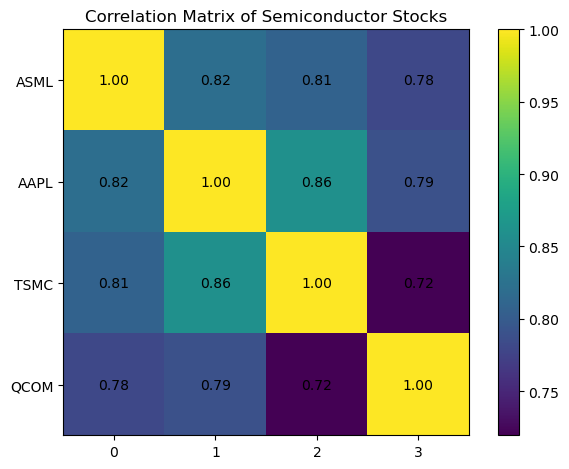
\includegraphics[width=0.8\linewidth]{group1-1.png}
        \caption{Correlation matrix of semiconductor stocks used in Model 1}
        \label{fig:my_image_label}
    \end{figure}
    
    The high VIFs suggest multicollinearity, which is economically expected: most major semiconductor firms are deeply interdependent through shared supply chains; Intel, for example, relies on TSMC for chip manufacturing (Reuters, 2025). This interdependence means these stocks move together, reducing their individual explanatory power. TSMC has the highest correlation with NVIDIA at 0.86, while others range from 0.72 to 0.82. Overall, sector-linked stocks are a reasonable indicator of the direction of NVIDIA's price movement but insufficient for precise estimation on their own.
    
    \begin{figure}[H]
        \centering
        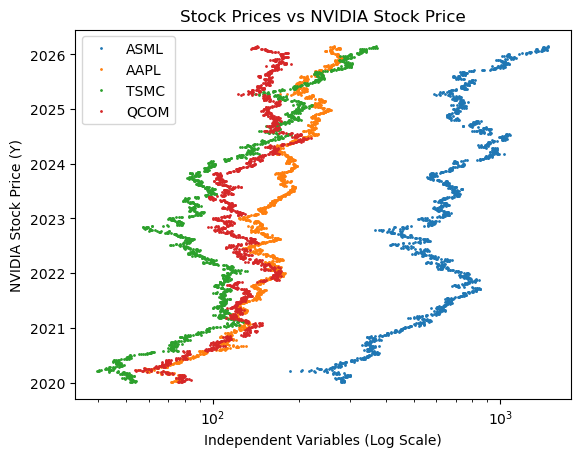
\includegraphics[width=0.9\linewidth]{group1.png}
        \caption{VIF plot for Model 1 regressors}
        \label{fig:my_image_label}
    \end{figure}
    
    \vspace{2em}
    
    \subsubsection{Model 2:}\label{sec:model2}
    
    Metal production volumes act as a supply-side cost input variable: NVIDIA's GPUs require copper, gold, silver, silicon, tin, aluminum, and rare earth elements. When the supply of these materials increases, input costs for chip manufacturers like TSMC may fall, theoretically reducing production costs and supporting NVIDIA's margins. Model 2 tests this relationship using yearly USGS production data. The coefficients are very small, reflecting the indirect and lagged nature of the supply-chain transmission:
    
    \begin{table}[h]
    \centering
    \begin{tabular}{lc}
    \hline
    \textbf{Metal} & \textbf{Coefficient} \\
    \hline
    Silver & -0.0001 \\
    Tin & -9.472e-07 \\
    Silicon& -7.556e-07 \\
    Aluminum & 1.33e-07 \\
    Rare Earths  & 3.648e-05 \\
    Gold & 0.0020 \\
    \hline
    \end{tabular}
    \caption{Regression Coefficients for Yearly Metal Production}
    \end{table}
    
    The adjusted $R^2$ is 0.815, below the ideal 0.95 threshold. The Breusch-Pagan (LM = 11.14, p $=$ 0.084) and White's test ($\chi^2$ = 19.0, p $=$ 0.39) both accept the null hypothesis of homoskedasticity, which is a notable strength. The Durbin--Watson statistic of 2.586 (p = 0.2904) provides no strong evidence of autocorrelation, suggesting the independence assumption holds reasonably well. However, the VIFs are high:
    
    \begin{table}[h]
    \centering
    \begin{tabular}{lc}
    \hline
    \textbf{Metal} & \textbf{VIF} \\
    \hline
    Silver & 17.446360 \\
    Tin & 2.037078 \\
    Silicon& 28.393788 \\
    Aluminum & 66.044190 \\
    Rare Earths  & 2.597244 \\
    Gold & 10.959539 \\
    \hline
    \end{tabular}
    \caption{VIFs for yearly metal production}
    \end{table}
    
    \begin{figure}[H]
        \centering
        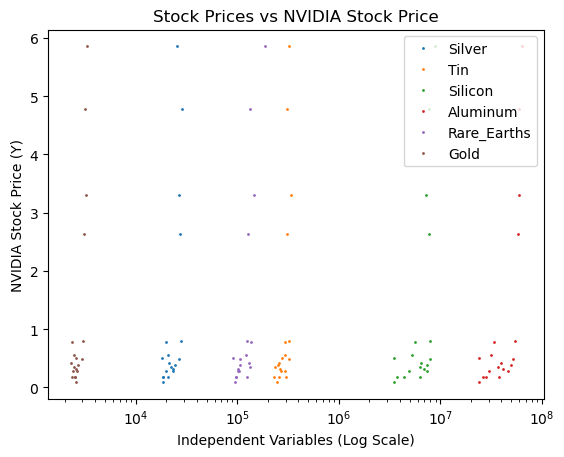
\includegraphics[width=0.7\linewidth]{group2.png}
        \caption{Scatter plot of yearly metal production vs NVIDIA close price}
        \label{fig:my_image_label}
    \end{figure}
    
    \begin{figure}[H]
        \centering
        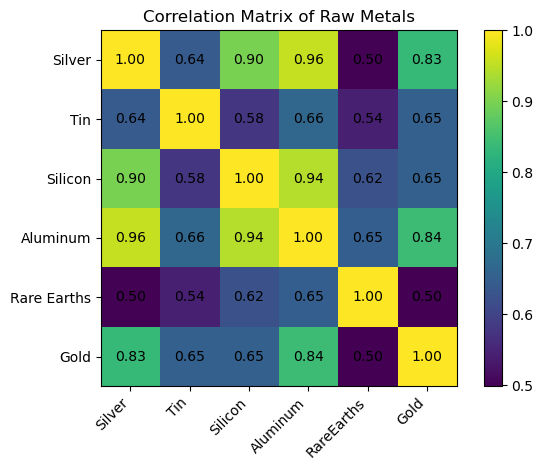
\includegraphics[width=0.8\linewidth]{group2-1.png}
        \caption{Correlation matrix of yearly metal production variables used in Model 2}
        \label{fig:my_image_label}
    \end{figure}
    
    The high VIFs are economically explained by the fact that global metal production trends tend to move together, driven by shared macroeconomic cycles, energy costs, and mining investment patterns. In Fig 7, the correlation between aluminum and silicon is 0.94, and aluminum and silver is 0.96, which explains why aluminum has the highest VIF at 66.04.
    
    \subsubsection{Model 3:}\label{sec:model3}
    
    Metal futures prices represent market expectations about future input costs, making them a forward-looking economic signal. A futures contract is an agreement to buy a commodity at a set price on a future date, used either for speculation or, more relevantly here, for hedging by manufacturers. TSMC, for example, could buy copper or gold futures contracts to lock in input prices and stabilise production costs. If futures prices rise, they signal expected cost increases for GPU production, which may compress NVIDIA's margins and weigh on its stock price.
    
    \begin{table}[h]
    \centering
    \begin{tabular}{lc}
    \hline
    \textbf{Metal Futures} & \textbf{Coefficient} \\
    \hline
    Copper & 12.8265 \\
    Gold & 0.0941 \\
    Silver  & -0.6901 \\
    Platinum & -0.0695 \\
    \hline
    \end{tabular}
    \caption{Regression Coefficients for Metals Futures}
    \end{table}
    
    For example, if copper futures change by \$1, NVIDIA's price changes by \$12.83, reflecting copper's central role in circuit board and chip packaging production. The model has an adjusted $R^2$ of 0.898. The Breusch-Pagan (LM = 512.00, p $<$ 0.001) and White's test ($\chi^2$ = 683.22, p $<$0.001) reject homoskedasticity; robust standard errors (HC3) were applied. The Durbin--Watson statistic of 0.034 signals severe serial autocorrelation, making standard errors unreliable, though coefficient estimates remain unbiased.
    
    \begin{table}[h]
    \centering
    \begin{tabular}{lc}
    \hline
    \textbf{Metal Futures} & \textbf{VIF} \\
    \hline
    Copper & 2.109996 \\
    Gold & 7.038074 \\
    Silver  & 18.195851 \\
    Platinum & 8.528261 \\
    \hline
    \end{tabular}
    \caption{VIF scores for Metals Futures}
    \end{table}
    
    \begin{figure}[H]
        \centering
        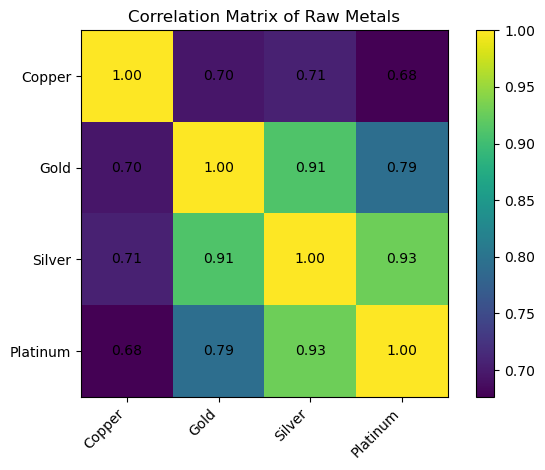
\includegraphics[width=0.9\linewidth]{group3-1.png}
        \caption{Correlation matrix of daily metal futures prices used in Model 3}
        \label{fig:my_image_label}
    \end{figure}
    
    Silver's high VIF is economically explained by its membership in the precious metals market alongside gold and platinum, as all three respond to similar macroeconomic forces such as inflation expectations and safe-haven demand. Copper's low VIF reflects its distinct industrial demand drivers, making it a more independent variable in this group.
    
    \subsubsection{Model 4:}\label{sec:model4}
    
    Metal ETFs (Exchange-Traded Funds) hold collections of commodity-related assets and thus reflect real-time market pricing of input costs. GLD, SLV, and PPLT hold physical gold, silver, and platinum respectively; CPER holds copper futures; and URA holds uranium mining stocks. Unlike yearly production data, ETFs capture daily investor sentiment around commodity markets, making them a more responsive economic signal.
    
    \begin{table}[h]
    \centering
    \begin{tabular}{lc}
    \hline
    \textbf{Metal ETFs} & \textbf{Coefficient} \\
    \hline
    Gold & 0.7520 \\
    Silver & -0.3677 \\
    Copper  & 0.4037 \\
    Platinum & -0.8809 \\
    Uranium & 2.4528 \\
    \hline
    \end{tabular}
    \caption{Regression Coefficients for Metal ETFs}
    \end{table}
    
    These coefficients have an adjusted $R^2$ value of 0.927. The metal with the largest coefficient is uranium (2.4528), which is economically significant: AI data centres require enormous amounts of electricity, and current electric grids are struggling to meet this demand. As a result, AI companies are increasingly investing in small modular nuclear reactors (SMRs) to power their data centres independently of the broader grid. Rising uranium prices therefore signal rising expected energy costs for AI infrastructure, directly affecting NVIDIA's growth outlook. The other metals are used in GPU production, NVIDIA's main product. Both the Breusch-Pagan (LM = 321.64, p $<$ 0.001) and White's test ($\chi^2$ = 555.78, p $<$0.001) reject homoskedasticity; robust standard errors (HC3) were applied. The Durbin--Watson statistic (0.049, p $\approx$ 0.0) reveals strong autocorrelation.
    
    \begin{table}[h]
    \centering
    \begin{tabular}{lc}
    \hline
    \textbf{Metal ETFs} & \textbf{VIFS} \\
    \hline
    Gold & 9.303403 \\
    Silver & 17.051093 \\
    Copper  & 3.061417 \\
    Platinum & 7.710108 \\
    Uranium & 6.072512 \\
    \hline
    \end{tabular}
    \caption{VIF scores for Metal ETFs}
    \end{table}
    
    \begin{figure}[H]
        \centering
        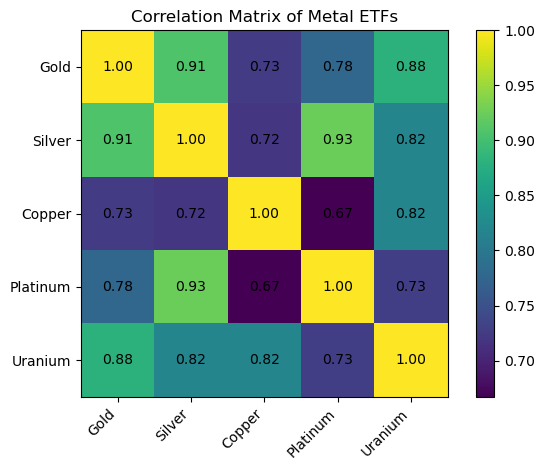
\includegraphics[width=0.9\linewidth]{group4-1.png}
        \caption{Correlation matrix of metal ETFs used in Model 4}
        \label{fig:my_image_label}
    \end{figure}
    
    As in Model 3, gold, silver, and platinum's high VIFs reflect their shared precious metals market dynamics. Copper's low VIF again reflects its industrial rather than speculative demand base.
    
    \subsubsection{Model 5:}\label{sec:model5}
    
    The S\&P 500 is a stock index tracking the 500 largest US companies by market capitalisation, widely considered the best single measure of overall US economic health. A rising S\&P 500 signals broad economic expansion, increasing corporate investment in technology, including AI infrastructure, which supports demand for NVIDIA's products. This investigation uses the daily percentage change of both series.
    
    \begin{table}[h]
    \centering
    \begin{tabular}{lc}
    \hline
    \textbf{Index} & \textbf{Coefficient} \\
    \hline
    S\&P 500 & 0.0524 \\
    \hline
    \end{tabular}
    \caption{Regression Coefficient for S\&P 500}
    \end{table}
    
    The coefficient of 0.0524 means that for every \$1 the S\&P 500 moves, NVIDIA moves \$0.0524 in the same direction. The adjusted $R^2$ of 0.901 means that about 90\% of NVIDIA's stock movements can be explained by the S\&P 500, which is remarkably high for a single variable. The Breusch-Pagan (LM = 142.03, p $<$ 0.001) and White's test ($\chi^2$ = 369.59, p $<$ 0.001) reject homoskedasticity; robust standard errors (HC3) were applied. The Durbin--Watson statistic of 0.040 (p $\approx$ 0.0) reveals strong autocorrelation. VIF = 1, as expected for a single-variable model. Despite a high $R^2$, the severe autocorrelation renders Model 5 unreliable for estimating NVIDIA's close price, as its explanatory power is trend-driven rather than genuinely predictive.
    
    \begin{figure}[H]
        \centering
        \includegraphics[width=0.9\linewidth]{group5.png}
        \caption{Scatter plot of S\&P 500 vs NVIDIA daily close price}
        \label{fig:my_image_label}
    \end{figure}
    
    \subsubsection{Model 6:}\label{sec:model6}
    
    The NASDAQ 100 index represents the 100 largest non-financial companies traded on the NASDAQ exchange, weighted by market capitalisation. Unlike the S\&P 500, it is concentrated in technology firms, making it a more targeted measure of the sector-wide conditions that drive NVIDIA's valuation. NVIDIA's current weight in the index is 12.96\% (as of 3/2/2026), meaning its own movements partly drive the index, which is a limitation worth noting. The adjusted $R^2$ is 0.910.
    
    \begin{table}[h]
    \centering
    \begin{tabular}{lc}
    \hline
    \textbf{Index} & \textbf{Coefficient} \\
    \hline
    NDX & 0.0124 \\
    \hline
    \end{tabular}
    \caption{Regression Coefficient for NASDAQ 100}
    \end{table}
    
    For every \$1 change in NDX, NVDA changes by \$0.0124 in the same direction. The Breusch-Pagan (LM = 81.89, p $<$ 0.001) and White's test ($\chi^2$ = 131.77, p $<$ 0.001) reject homoskedasticity; robust standard errors (HC3) were applied. The Durbin--Watson statistic of 0.045 (p $\approx$ 0.0) provides strong evidence of autocorrelation. VIF = 1. Despite a high $R^2$ of 0.910, the severe autocorrelation renders Model 6 unreliable for estimating NVIDIA's close price.
    
    \begin{figure}[H]
        \centering
        \includegraphics[width=0.9\linewidth]{group6-1.png}
        \caption{Scatter plot of NASDAQ 100 vs NVIDIA daily close price}
        \label{fig:my_image_label}
    \end{figure}
    
    \subsubsection{Model 7:}\label{sec:model7}
    
    AI data centres require high and growing amounts of electricity, but current electric grids are struggling to meet demand. This has created a new derived demand for energy solutions, with major AI companies such as Google, Meta, and OpenAI investing in small modular reactors (SMRs) and micro modular reactors (MMRs) to power their data centres. Since NVIDIA's growth is directly tied to AI infrastructure expansion, the valuations of these energy firms are economically linked to NVIDIA's own prospects. Oklo, for example, is an American company developing SMRs (up to 300 MW), while Nano Nuclear develops MMRs (typically under 10--20 MW) intended to be placed next to data centres to ensure energy security and reduce grid dependence.
    
    \begin{table}[h]
    \centering
    \begin{tabular}{lc}
    \hline
    \textbf{SMR and MMR Company Stocks} & \textbf{Coefficients} \\
    \hline
    NuScale & 0.3682 \\
    Oklo & -0.0811 \\
    GE Vernova   & 0.0176 \\
    BWX & 0.6739 \\
    Nano Nuclear  & 0.0078 \\
    \hline
    \end{tabular}
    \caption{Coefficients for SMR and MMR Company Stocks}
    \end{table}
    
    These coefficients, along with an adjusted $R^2$ of 0.906, show a strong relationship between nuclear energy stocks and NVIDIA's price, consistent with the view that NVIDIA's valuation increasingly reflects broader AI infrastructure investment rather than semiconductor fundamentals alone. The Breusch-Pagan (LM $\approx$ 49.07, p $<$ 0.001) and White's test ($\chi^2$ = 138.58, p $<$ 0.001) reject homoskedasticity; robust standard errors (HC3) were applied. The Durbin--Watson statistic of 0.170 (p $\approx$ 0.0) indicates positive autocorrelation.
    
    \begin{table}[h]
    \centering
    \begin{tabular}{lc}
    \hline
    \textbf{SMR and MMR Company Stocks} & \textbf{VIFS} \\
    \hline
    NuScale & 3.252240 \\
    Oklo & 9.275726 \\
    GE Vernova   & 7.662576 \\
    BWX & 10.590868 \\
    Nano Nuclear  & 5.090562 \\
    \hline
    \end{tabular}
    \caption{VIFs for SMR and MMR Company Stocks}
    \end{table}
    
    \begin{figure}[H]
        \centering
        \includegraphics[width=0.8\linewidth]{group7-1.png}
        \caption{Correlation matrix of SMR and MMR company stocks used in Model 7}
        \label{fig:my_image_label}
    \end{figure}
    
    The high VIFs are economically expected: all five companies operate in the same niche energy market and respond to the same policy signals, uranium prices, and energy sector trends. NuScale's relatively low VIF reflects its more distinct market position as the only firm to have received Nuclear Regulatory Commission approval, differentiating it from competitors.
    
    \subsubsection{Model Composite: A Synthesis of Optimal Parameters}\label{sec:modelu}
    
    Model Composite combines parameters from Models 1, 4, and 6, selected for their low VIFs, high adjusted $R^2$, and strong diagnostic test results. Economically, the three variables capture distinct transmission channels: ASML represents supply-chain cost and technology access constraints in semiconductor manufacturing; the Uranium ETF captures the energy infrastructure investment thesis driving AI demand; and the NASDAQ 100 reflects aggregate technology sector sentiment.
    
    \begin{table}[h]
    \centering
    \begin{tabular}{lc}
    \hline
    \textbf{Parameter} & \textbf{Coefficient} \\
    \hline
    ASML & -0.0803 \\
    Uranium ETF   & 1.2540 \\
    Nasdaq 100 & 0.0131 \\
    \hline
    \end{tabular}
    \caption{Model Composite Coefficients with Newey-West Standard Errors}
    \end{table}
    
    The adjusted $R^2$ is 0.932. The uranium ETF's dominant coefficient (1.254) reflects how NVIDIA's valuation has evolved into a broader bet on AI infrastructure rather than traditional semiconductor fundamentals; rising uranium prices signal expanding energy investment in AI, which drives demand for NVIDIA's GPUs. The Breusch-Pagan (LM = 187.45, p $<$ 0.001) and White's test ($\chi^2$ = 609.77, p $<$ 0.001) reject homoskedasticity. Newey-West (HAC) standard errors with 8 lags were applied to account for both heteroskedasticity and autocorrelation, with all coefficients remaining highly significant (p $<$ 0.001). The Durbin-Watson statistic of 0.024 indicates severe autocorrelation, common in financial time series.
    
    \begin{table}[h]
    \centering
    \begin{tabular}{lc}
    \hline
    \textbf{Parameter} & \textbf{VIF} \\
    \hline
    ASML & 4.179405 \\
    Uranium ETF   & 7.562880 \\
    Nasdaq 100 & 7.107493 \\
    \hline
    \end{tabular}
    \caption{VIFs for Model Composite}
    \end{table}
    
    \begin{figure}[H]
        \centering
        \includegraphics[width=0.9\linewidth]{groupU-1.png}
        \caption{Correlation matrix of Model Composite parameters: ASML, Uranium ETF, and NASDAQ 100}
        \label{fig:my_image_label}
    \end{figure}
    
    The high correlation (0.92) between the uranium ETF and the NASDAQ 100 is economically intuitive: technology companies, which dominate the NASDAQ, are among the largest consumers of energy, meaning rising energy investment and rising tech valuations tend to move together.
    
    \section{Conclusion}
    
    \subsection{Model Results}
    
    Overall, the models can be by their practical reliability for financial estimation. The strongest model, Model 2; has an $R^2$ of 0.815, the best Durbin-Watson result (2.586, p = 0.29), and acceptable Breusch-Pagan and White's test results, with its only weakness being high VIF scores; it has the best determination power. (see \ref{sec:model2}). Model 7 and Model Composite had severe autocorrelation but after the Cochrane-Orcutt procedure returned much improved Durbin-Watson statistics of 2.0387 and 2.0507 respectively, though with lower adjusted $R^2$s of 0.4613 and 0.4459, thus their determination power is only moderate (see \ref{sec:model7} and \ref{sec:modelu}). The remaining models (1, 3, 4, 5, and 6) all have strong $R^2$ values (0.898 to 0.932) but are severely undermined by Durbin-Watson statistics ranging from 0.034 to 0.170, and Cochrane-Orcutt correction reduces their $R^2$ to near zero which diminishes their determination power. (see \ref{sec:model1}, \ref{sec:model3}, \ref{sec:model4}, \ref{sec:model5}, \ref{sec:model6}).
    
    \subsection{Answering the Research Question}
    
    NVIDIA's stock close price can be estimated with linear regression, but only to a moderate extent. After applying the Cochrane-Orcutt procedure to correct for autocorrelation, the best-performing models (Model 7 and Model Composite) retained adjusted $R^2$ values of 0.461 and 0.446 respectively, meaning the x-variables explain approximately 45\% of NVIDIA's price movements when the time-series structure of the data is properly accounted for.w
    
    This finding is consistent with Fama's (1970) Efficient Market Hypothesis (EMH), which holds that asset prices in competitive markets fully reflect all publicly available information at any given time. Under the semi-strong form of the EMH, no model using publicly available variables, such as those used in this investigation, should be able to systematically and reliably estimate future prices, since that information is already priced in by rational, profit-seeking market participants. The residual explanatory power retained by the corrected models likely reflects shared macroeconomic trends rather than genuine price discovery.
    
    From a microeconomic standpoint, NVIDIA operates in a market characterised by highly inelastic short-run supply: GPU production depends on a complex global supply chain involving specialised inputs, including lithography equipment from ASML, chip fabrication from TSMC, and critical metals such as copper and rare earths, which cannot be rapidly scaled in response to demand changes. Meanwhile, demand for NVIDIA's GPUs has grown rapidly and inelastically, driven by AI adoption across industries. This supply-demand imbalance means NVIDIA's price is highly sensitive to idiosyncratic shocks, such as export restrictions, earnings surprises, or new product announcements, which are not captured by any of the external market variables used in this investigation, and which no linear regression model of this type could systematically estimate.
    
    Furthermore, NVIDIA's valuation increasingly reflects speculative demand: investors price in expected future AI adoption, meaning the stock behaves partly as a financial asset driven by expectations and sentiment rather than current fundamentals alone (Malhotra \& Tandon, 2013). This speculative component further limits the reliability of regression-based estimation.
    
    A more appropriate econometric approach for this type of data would be an Autoregressive Integrated Moving Average (ARIMA) model, which explicitly models the time-series structure of prices rather than requiring post-hoc corrections such as Cochrane-Orcutt. In economic terms, ARIMA treats past prices as informative signals about future prices, reflecting the role of adaptive expectations in financial markets, making it better suited to capturing the dynamics of a stock as idiosyncratic as NVIDIA's.

    \newpage

%TC:ignore
\section{Bibliography}
    
Fama, E. F. (1970). Efficient capital markets: A review of theory and empirical work. \textit{Journal of Finance, 25}(2), 383--417.

Gujarati, D. N. (2011). \textit{Econometrics by example}. Palgrave Macmillan.

Malhotra, N., \& Tandon, K. (2013). \textit{Determinants of stock prices: Empirical evidence from NSE 100 companies}. \textit{International Journal of Research in Management \& Technology, 3}(3), 86--90.

Oklo Inc. (n.d.). \textit{About Oklo}. Oklo. \url{https://oklo.com/about/default.aspx}

R1B0PR07008. (2026). \textit{Clean Data Fixed from Model 7.ipynb} (Version from School-Public repository) [Jupyter Notebook]. GitHub. \url{https://github.com/R1B0PR07008/School-Public/blob/main/Extended%20Essay/Clean%20Data%20Fixed%20from%20Model%207.ipynb}

Reuters. (2025, August 5). \textit{Intel struggles with key manufacturing process for next PC chip, sources say}. Reuters. \url{https://www.reuters.com/world/asia-pacific/intel-struggles-with-key-manufacturing-process-next-pc-chip-sources-say-2025-08-05/}

U.S. Geological Survey. (n.d.). \textit{Aluminum statistics and information}. U.S. Department of the Interior. \url{https://www.usgs.gov/centers/national-minerals-information-center/aluminum-statistics-and-information}

U.S. Geological Survey. (n.d.). \textit{Copper statistics and information}. U.S. Department of the Interior. \url{https://www.usgs.gov/centers/national-minerals-information-center/copper-statistics-and-information}

U.S. Geological Survey. (n.d.). \textit{Gold statistics and information}. U.S. Department of the Interior. \url{https://www.usgs.gov/centers/national-minerals-information-center/gold-statistics-and-information}

U.S. Geological Survey. (n.d.). \textit{Platinum-group metals statistics and information}. U.S. Department of the Interior. \url{https://www.usgs.gov/centers/national-minerals-information-center/platinum-group-metals-statistics-and-information}

U.S. Geological Survey. (n.d.). \textit{Rare earths statistics and information}. U.S. Department of the Interior. \url{https://www.usgs.gov/centers/national-minerals-information-center/rare-earths-statistics-and-information}

U.S. Geological Survey. (n.d.). \textit{Silicon statistics and information}. U.S. Department of the Interior. \url{https://www.usgs.gov/centers/national-minerals-information-center/silicon-statistics-and-information}

U.S. Geological Survey. (n.d.). \textit{Silver statistics and information}. U.S. Department of the Interior. \url{https://www.usgs.gov/centers/national-minerals-information-center/silver-statistics-and-information}

Wooldridge, J. M. (2012). \textit{Introductory econometrics: A modern approach} (5th ed.). South-Western Cengage Learning.

Yahoo Finance. (n.d.). \textit{Yahoo Finance}. Yahoo. \url{https://finance.yahoo.com/}
%     %TC:endignore
    
    \end{document}